\documentclass[tikz,border=5pt]{standalone}
\usepackage{amsmath}

\definecolor{corba}{HTML}{365FB3}
\definecolor{mesura}{HTML}{B91C1C}
\definecolor{accent}{HTML}{7C3AED}
\definecolor{fons}{HTML}{F4F7FC}

\tikzset{
  cara/.style={draw=corba, very thick, fill=corba!9, line join=round},
  vora/.style={draw=corba, very thick, line join=round},
  oculta/.style={draw=corba!55, densely dashed, line width=.8pt},
  cota/.style={<->, >=stealth, draw=mesura, semithick},
  etiqueta/.style={text=mesura, font=\small},
}

\begin{document}
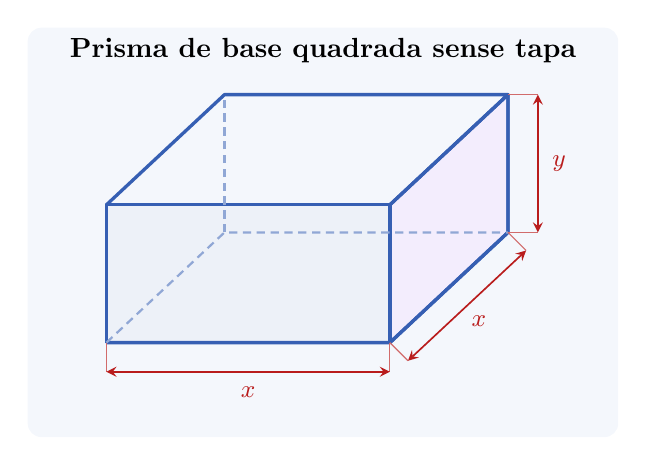
\begin{tikzpicture}[x=1cm,y=1cm]
  \fill[rounded corners=5pt, fons] (-.45,-.65) rectangle (7.05,4.55);

  % Vèrtexs d'un prisma recte de base quadrada.
  \coordinate (A) at (0.55,0.55);
  \coordinate (B) at (4.15,0.55);
  \coordinate (C) at (5.65,1.95);
  \coordinate (D) at (2.05,1.95);
  \coordinate (E) at (0.55,2.30);
  \coordinate (F) at (4.15,2.30);
  \coordinate (H) at (2.05,3.70);
  \coordinate (G) at (5.65,3.70);

  % Cares visibles del prisma. La cara superior no es dibuixa perquè
  % la capsa és oberta.
  \filldraw[cara] (A)--(B)--(F)--(E)--cycle;
  \filldraw[cara, fill=accent!9] (B)--(C)--(G)--(F)--cycle;

  % Contorn superior obert i arestes visibles.
  \draw[vora] (A)--(B)--(C)--(G);
  \draw[vora] (A)--(E)--(F)--(B);
  \draw[vora] (E)--(H)--(G)--(F);

  % Arestes posteriors ocultes, dibuixades amb traç discontinu.
  \draw[oculta] (A)--(D)--(C);
  \draw[oculta] (D)--(H);

  % Cotes.
  \draw[mesura!65] (A)--(0.55,0.18) (B)--(4.15,0.18);
  \draw[cota] (0.55,0.18)--(4.15,0.18);
  \node[etiqueta] at (2.35,-.08) {$x$};
  \draw[mesura!65] (B)--(4.38,.32) (C)--(5.88,1.72);
  \draw[cota] (4.38,.32)--(5.88,1.72);
  \node[etiqueta] at (5.28,.82) {$x$};
  \draw[mesura!65] (C)--(6.03,1.95) (G)--(6.03,3.70);
  \draw[cota] (6.03,1.95)--(6.03,3.70);
  \node[etiqueta] at (6.30,2.83) {$y$};

  \node[font=\bfseries] at (3.30,4.26) {Prisma de base quadrada sense tapa};
\end{tikzpicture}
\end{document}
